\documentclass[a4paper,12pt]{article}
\usepackage[utf8]{inputenc}
\usepackage[spanish]{babel}
\usepackage{geometry}
\geometry{margin=2.5cm}
\usepackage{graphicx}
\usepackage{amsmath, amssymb}
\usepackage{xcolor}
\usepackage{tikz, tcolorbox}
\usepackage{listings}
\usepackage{fancyvrb}
\usepackage{hyperref}
\usepackage{float}

\title {
\includegraphics[width=0.4\textwidth]{Ing_Uni.jpg}\\[2ex]{\textbf{Informe Proyecto\\ Restaurante}\\[1.5ex] Programacion II\\[20ex]}}
\author{Diego Hernandez, Benjamin Soto, Eduardo Necul}
\date{Octubre 2025}

\lstset{
    backgroundcolor=\color{gray!10},
    basicstyle=\ttfamily\footnotesize,
    frame=single,
    breaklines=true,
    keywordstyle=\color{blue},
    commentstyle=\color{green!50!black},
    stringstyle=\color{orange},
    showstringspaces=false
}

\begin{document}

\maketitle

\newpage
\tableofcontents
\newpage

\section{Introduccion}

Se nos hizo entrega un codigo base para la funcion de un restaurante incompleto, en cual nosotros debemos encargarnos de completarlo y refinarlo con la forma de programar \textbf{POO} (programacion orientada a objetos), sin salirnos de las casillas del esqueleto inicial. Ademas nos preocuparemos de explicar cada cambio aplicado al codigo, que utilidad le dimos a las funciones vacias y el diagrama de clases en base a este.

\section{Cambios y implementaciones}

Apartado donde nos centraremos en explicar que modificamos en el codigo para su mejor comprension y funcionalidad.

\subsection{Diagrama de Clases del problema}

Para visualizar con claridad el problema presentado y su diseño \textbf{POO}, diseñamos un diagrama UML con el objetivo de visualizar las distintas clases utilizadas y sus interrelaciones a través de relaciones (asociación, agrupación, composición) y cardinalidades.

\begin{figure}[H]
    \centering
    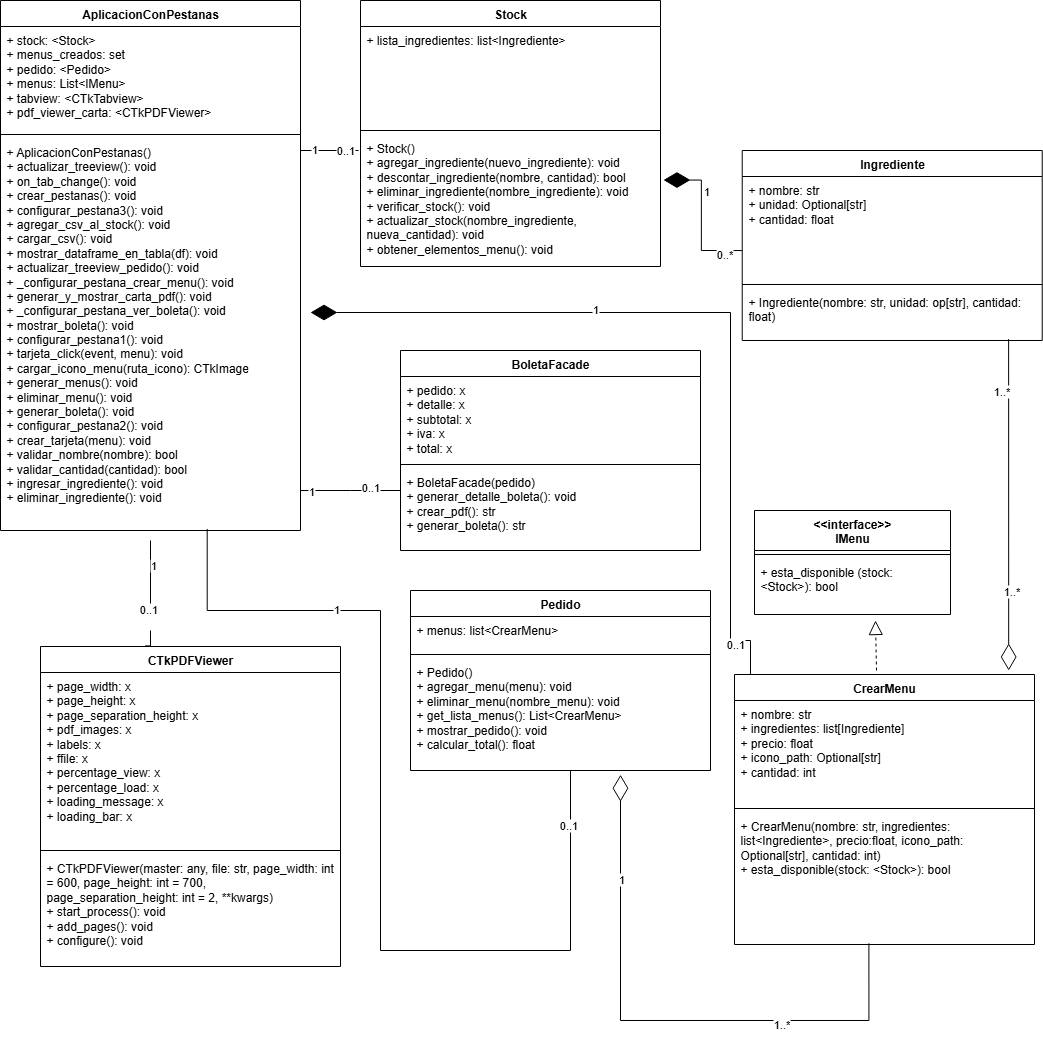
\includegraphics[width=1.1\textwidth]{Diagrama-Restaurante.drawio.png}
    \caption{Diagrama de Clases de la aplicación.}.
\end{figure}



La clase \textbf{\textit{AplicacionConPestanas}} es la principal clase del programa, ya que es ella la que se usa para configurar la interfaz de CustomTkinter e instanciar, relacionar y modificar el resto de clases del sistema, las cuales se describen a continuación brevemente:
\begin{itemize}

    \item La clase \textit{Stock} es aquella donde se administra la información de ingredientes, y que servirá para determinar la disponibilidad de menúes (o platos) en función de si existen los ingredientes requeridos o no, y tiene una relación de asociación con \textit{AplicacionConPestanas}, ya que pese a que esta última instancia un objeto Stock, no hay un contenedor de los objetos instanciados (lista) y ambas clases son independientes, en la que una referencia a otra.
    
    \item La clase \textit{Ingrediente} es aquella que configura la información de un ingrediente en base a sus tres atributos principales y que coinciden con el estándar de información del archivo CSV. Es el elemento principal de la clase Stock.
    
    \item La clase \textit{CrearMenu} es donde se configura la información de un menú/platillo y se configura en base a objetos Ingredientes, debido a la relación explicada en la clase Stock.
    \begin{itemize}
        \item[$\rightarrow$] Debido a la relación entre Stock y menúes, los objetos CrearMenu tienen una relación de agregación con los objetos Ingrediente, ya que toman ingredientes determinados y los configuran como parte de sus requisitos (los ingredientes requeridos o que forman parte de CrearMenu deben coincidir con ingredientes existentes en Stock).
        \item[$\rightarrow$] Exclusivamente, esta clase cuenta con una relación de abstracción + implementación con la clase IMenu, la cual corresponde a una interfaz que verifica que la construcción de CrearMenu cumpla los criterios solicitados.
    \end{itemize}
    
    \item La clase \textit{Pedido} es la clase donde se configura la información del pedido de un cliente en particular.
    
        \begin{itemize}
            \item[$\rightarrow$] La aplicación solo puede trabajar con máximo un Pedido a la vez, o con carencia de este, esto en una relación de asociación, ya que la existencia de ambos es bastante independiente (salvo por la instanciación que depende AplicacionConPestanas).
            \item[$\rightarrow$] La clase Pedido se configura en base a los menúes (CrearMenu) instanciados, y los va agregando en sí, teniendo la posibilidad de tener 1 o muchos menúes (de lo contrario Pedido estaría vacío y no habría datos con los que trabajar).
        \end{itemize}
        
    \item La clase \textit{BoletaFacade} tiene el proposito de generar la boleta de compra a partir de la recepcion de un objeto "pedido", pedido cual contiene lo comprado por el cliente en el restaurant.
    
    \item La clase \textit{CtkPDFViewer} es una clase auxiliar que sirve para crear la visualización del archivo PDF con la función de carga de PDF de \textit{AplicacionConPestanas}.
\end{itemize}

\subsection{Cambios de variable o definiciones}

\begin{lstlisting}[language=Python, caption={Cambios de definiciones o variables}, frame=single]
def actualizar_treeview => def actualizar_treeview_stock
def configurar_pestana1 => def configurar_pestana_stock
def configurar_pestana2 => def configurar_pestana_pedido
def configurar_pestana3 => def configurar_pestana_CSV
self.treeview_menu => self.treeview_pedido
tarjetas_frame => self.frame_tarjetas
self.entry_unidad => self.combo_unidad
\end{lstlisting}

Basicamente, la mayoria de los cambios de funciones o variables es para no perdernos en el codigo y saber precisamente que parte del codigo estamos modificando. Ademas cuando modificamos una variable adaptar ese cambio cada parte del codigo que afecte.

\subsection{Implementaciones de codigo}

Entraremos a mas profundidad sobre el codigo nuevo o nuevas funciones que se aplicaron para la utilidad de nuestro proyecto, explicando el porque y que hacen.

\begin{lstlisting}[language=Python, caption={Implementaciones de codigo}, frame=single]
# antes
def actualizar_treeview(self):
    pass
# despues
def actualizar_treeview_stock(self):
    self.treeview_stock.delete(*self.treeview_stock.get_children())
        for ingrediente in sorted(self.stock.lista_ingredientes, key=lambda item: item.nombre):
            self.treeview_stock.insert("", "end", values=(
                ingrediente.nombre, ingrediente.unidad, ingrediente.cantidad))
\end{lstlisting}

Se rellena codigo vacio para darle una utilidad especifica a la pestaña stock porque mas adelante de implemento una funcion que se podria confundir, entonces:

\begin{itemize}
    \item Se le da un nombre mas especifico, para no confundir.
    \item Borra completamente la tabla cada que se actualiza para evitar que se dupliquen ingredientes con \verb|self.treeview_stock.delete(...)|
    \item Se ordenan los ingredentes de forma alfabetica para una demostracion mas ordenada y profesional, con \verb|sorted(...)|
    \item Se rellena la tabla con informacion reciente obtenida por\\ \verb|self.stock.lista_ingredientes|
\end{itemize}
Con todas estas funcionalidades se logra una funcion correcta,limpia y ordena para la pestaña stock.
\newpage
\begin{lstlisting}[language=Python, caption={Implementaciones de codigo}, frame=single]
# antes
def generar_menus(self):
    pass
# despues
def generar_menus(self):
    for tarjeta in self.frame_tarjetas.winfo_children():
        tarjeta.destroy()
    listaMenus = get_default_menus()
    columna = 0
    for menu in listaMenus:
        if menu.esta_disponible(self.stock):
            columna += 1
            self.crear_tarjeta(menu, columna)
\end{lstlisting}
\textbf{Utilidades destacadas:}
\begin{itemize}
    \item \verb|for tarjeta in self.frame_tarjetas.winfo_children(): tarjeta.destroy()|\\es un bucle el cual recorre todos los elementos que ya existen dentro de\\ \verb|self.frame_tarjetas| y los borra para una limpieza.
    \item \begin{lstlisting}
        listaMenus = get_default_menus()
        ...
        for menu in listaMenus:
            if menu.esta_disponible(self.stock):
                ...
    \end{lstlisting}
    Esta es la mas importante del bloque ya que recorre todos los menus disponibles por el restaurante formando una lista. Para despues verificar si lo puede preparar.
    \item \begin{lstlisting}
        columna = 0
        ...
            if menu.esta_disponible(self.stock):
                columna += 1
                self.crear_tarjeta(menu, columna)
    \end{lstlisting}
    Por cada menú que SÍ está disponible, incrementa un contador \verb|(columna)| y luego llama a la función \verb|self.crear_tarjeta| para que dibuje la tarjeta en la pantalla.
\end{itemize}

\newpage

\begin{lstlisting}[language=Python, caption={Implementaciones de codigo}, frame=single]
    def ingresar_ingrediente(self):
        nombre = self.entry_nombre.get()
        unidad = self.combo_unidad.get()
        cantidad = self.entry_cantidad.get()

        if not self.validar_nombre(nombre) or not self.validar_cantidad(cantidad):
            return

        ingrediente_a_agregar = Ingrediente(nombre, unidad, float(cantidad))

        self.stock.agregar_ingrediente(ingrediente_a_agregar)

        self.entry_nombre.delete(0, 'end')
        self.entry_cantidad.delete(0, 'end')

        self.actualizar_treeview_stock()
\end{lstlisting}
Funcion importante que bien ya sabiendo por su nombre, cumple con la utilidad de que funcione el boton de \textbf{Ingresar ingrediente} en la pestaña de stock, cumpliendo con el requerimiento de que se pueda ingresar cualquier ingrediente correctamente.

\textbf{1. Recopilacion de Datos de la Interfaz}\\
En esta etapa, se obtienen los valores que el usuario ha introducido en los campos de la interfaz gráfica.
\begin{lstlisting}[language=Python, caption={desenglosando codigo}, frame=single]
nombre = self.entry_nombre.get()
unidad = self.combo_unidad.get()
cantidad = self.entry_cantidad.get()
\end{lstlisting}
\begin{itemize} \item \verb|self.entry_nombre.get()|: Captura el texto del campo de entrada del nombre. \item \verb|self.combo_unidad.get()|: Obtiene la opción seleccionada ("unid" o "kg") del menú desplegable. \item \verb|self.entry_cantidad.get()|: Captura el texto del campo de entrada de la cantidad. 
\end{itemize}
\textbf{2. Validacion de la Entrada}\\
Antes de procesar los datos, se verifica que cumplan con las reglas de negocio definidas (ej. el nombre es válido y la cantidad es un número positivo)
\begin{lstlisting}[language=Python, caption={desenglosando codigo}, frame=single]
    if not self.validar_nombre(nombre) or not self.validar_cantidad(cantidad):
    return
\end{lstlisting}

\begin{itemize} \item La condición \verb|if| evalúa el resultado de los métodos de validación. Si alguno de ellos retorna \verb|false|, la palabra clave \verb|return| detiene la ejecución del método para prevenir el ingreso de datos corruptos al sistema. \end{itemize}

\newpage
\textbf{3. Procesamiento y Logica de Negocio}\\
Una vez que los datos son validados, se crea un objeto formal y se actualiza el estado del inventario.

\begin{lstlisting}[language=Python, caption={desenglosando codigo}, frame=single]
    ingrediente_a_agregar = Ingrediente(nombre, unidad, float(cantidad))
    self.stock.agregar_ingrediente(ingrediente_a_agregar)
\end{lstlisting}
\begin{itemize} 
\item \verb|Ingrediente(...)|: Se instancia un nuevo objeto de la clase Ingrediente. La cantidad, que es un texto (\textit{string}), se convierte a un número de punto flotante (\verb|float|) para permitir operaciones matemáticas. 
\item \verb|self.stock.agregar_ingrediente(...)|: Se invoca el método del objeto stock para añadir el nuevo ingrediente a la lista del inventario en la memoria del programa. 
\end{itemize}

\textbf{4. Actualizacion de la Interfaz Grafica}\\
Finalmente, se actualiza la vista para que el usuario pueda ver los resultados de su acción.

\begin{lstlisting}[language=Python, caption={desenglosando codigo}, frame=single]
    self.entry_nombre.delete(0, 'end')
    self.entry_cantidad.delete(0, 'end')
    self.actualizar_treeview_stock()
\end{lstlisting}

\begin{itemize} 
\item \verb|self.entry_*.delete(...)|: Se limpian los campos de entrada de texto para dejarlos listos para un nuevo ingreso. 
\item \verb|self.actualizar_treeview_stock()|: Se llama al método encargado de refrescar la tabla (\textit{Treeview}) del stock. Este método borra el contenido actual de la tabla y la vuelve a dibujar con la lista de ingredientes actualizada, reflejando así el cambio realizado. 
\end{itemize}

\textbf{funcion eliminar ingrediente}\\
Este bloque de código define el método \verb|eliminar_ingrediente|, cuya función es remover un ingrediente seleccionado por el usuario de la tabla de inventario y de la estructura de datos subyacente. El proceso se ejecuta en una secuencia lógica para garantizar la integridad de los datos y una correcta retroalimentación visual.
\begin{lstlisting}[language=Python, caption={implementacion de codigo}, frame=single]
def eliminar_ingrediente(self):
        item_seleccionado = self.treeview_stock.focus()
        if not item_seleccionado:
            CTkMessagebox(
                title="Aviso", message="Debes seleccionar un ingrediente de la tabla.", icon="warning")
            return

        detalles_item = self.treeview_stock.item(item_seleccionado)
        nombre_a_eliminar = detalles_item['values'][0]

        self.stock.eliminar_ingrediente(nombre_a_eliminar)
        self.actualizar_treeview_stock()
\end{lstlisting}

\newpage
\textbf{1. Identificacion del Elemento Seleccionado}\\
El primer paso consiste en identificar qué fila de la tabla (Treeview) ha seleccionado el usuario.
\begin{lstlisting}[language=Python, caption={desenglosando codigo}, frame=single]
    item_seleccionado = self.treeview_stock.focus()
\end{lstlisting}

\begin{itemize} 
\item El metodo \verb|focus()| del widget Treeview devuelve el identificador único del item que tiene el foco actual, es decir, el que está seleccionado. Si no hay ninguna selección, devuelve una cadena vacía. \end{itemize}

\textbf{2. Validacion de la Selección}\\
Se realiza una comprobacion para asegurar que el usuario ha seleccionado un ítem antes de proceder.
\begin{lstlisting}[language=Python, caption={desenglosando codigo}, frame=single]
    if not item_seleccionado:
            CTkMessagebox(
                title="Aviso", message="Debes seleccionar un ingrediente de la tabla.", icon="warning")
            return
\end{lstlisting}
\begin{itemize} 
\item Si la variable \verb|item_seleccionado| esta vacia, la condicion \verb|if| se evalua como verdadera. 
\item Se muestra una ventana emergente (\verb|CTkMessagebox|) para notificar al usuario que debe seleccionar un ingrediente. 
\item La instrucción \verb|return| detiene la ejecución del método para evitar errores. 
\end{itemize}
\textbf{3. Extracción del Nombre del Ingrediente}\\
Una vez validada la selección, se extrae el nombre del ingrediente que se desea eliminar.
\begin{lstlisting}[language=Python, caption={desenglosando codigo}, frame=single]
    detalles_item = self.treeview_stock.item(item_seleccionado)
    nombre_a_eliminar = detalles_item['values'][0]
\end{lstlisting}
\begin{itemize} 
\item \verb|self.treeview_stock.item(...)|: Este método retorna un diccionario con toda la información de la fila seleccionada. 
\item La clave \verb|'values'| de este diccionario contiene una tupla con los valores de cada columna (Nombre, Unidad, Cantidad). 
\item Se accede al primer elemento de esta tupla, \verb|[0]|, que corresponde al nombre del ingrediente. 
\end{itemize}
\newpage

\textbf{4. Ejecución de la Lógica de Negocio}\\
Con el nombre del ingrediente, se invoca al método correspondiente en el objeto stock para eliminarlo de la lista de datos en memoria.
\begin{lstlisting}[language=Python, caption={desenglosando codigo}, frame=single]
    self.stock.eliminar_ingrediente(nombre_a_eliminar)
\end{lstlisting}
\begin{itemize} 
\item Este es el paso donde se modifica el modelo de datos del programa, eliminando el objeto Ingrediente de la lista de inventario. 
\end{itemize}

\textbf{5. Actualización de la Interfaz Gráfica}\\
Finalmente, se refresca la tabla para que el cambio sea visible para el usuario.
\begin{lstlisting}[language=Python, caption={desenglosando codigo}, frame=single]
    self.actualizar_treeview_stock()
\end{lstlisting}
\begin{itemize} 
\item Se llama al método \verb|actualizar_treeview_stock()|, el cual se encarga de borrar el contenido actual de la tabla y redibujarlo con la lista de ingredientes actualizada, reflejando así la eliminación. 
\end{itemize}
\textbf{Funcion editar cantidad stock}
\begin{lstlisting}[language=Python, caption={Nuevo codigo}, frame=single]
    def editar_cantidad_stock(self, event):
        # 1. Identifica la fila en la que se hizo doble clic
        item_seleccionado = self.treeview_stock.focus()
        if not item_seleccionado:
            return

        # 2. Obtiene los detalles del ingrediente de esa fila
        detalles_item = self.treeview_stock.item(item_seleccionado)
        nombre_ingrediente = detalles_item['values'][0]
        cantidad_actual = detalles_item['values'][2]

        # 3. Abre una ventana emergente para pedir la nueva cantidad
        dialogo = ctk.CTkInputDialog(
            text=f"Ingrese la nueva cantidad para '{nombre_ingrediente}':",
            title="Actualizar Stock"
        )

        nueva_cantidad_str = dialogo.get_input()

        # 4. Si el usuario ingreso un valor y no cancelo
        if nueva_cantidad_str:
            try:
                nueva_cantidad = float(nueva_cantidad_str)
                if nueva_cantidad < 0:  # No permitir cantidades negativas
                    raise ValueError

                # 5. Llama a la funcion de la logica del Stock
                self.stock.actualizar_stock(nombre_ingrediente, nueva_cantidad)

                # 6. Refresca la tabla para mostrar el cambio
                self.actualizar_treeview_stock()

            except (ValueError, TypeError):
                CTkMessagebox(
                    title="Error", message="Por favor, ingrese un numero valido y positivo.", icon="cancel")
\end{lstlisting}

Basicamente despliega una ventana al hacer doble clic sobre un ingrediente, para poder editar su stock de una manera mas comoda, sin necesidad de estar ingresando ese mismo ingrediente varias veces con el boton.\\

\textbf{Funcion mostrar lista de compras}\\

\begin{lstlisting}[language=Python, caption={Nuevo codigo}, frame=single]
    def mostrar_lista_compras(self):
        # 1. Llama a la nueva funcion de la logica del Stock
        ingredientes_bajos = self.stock.obtener_elementos_menu(
            umbral=5)  # Puedes cambiar el umbral

        # 2. Prepara el mensaje para el usuario
        if not ingredientes_bajos:
            mensaje = "Excelente No hay ingredientes con bajo stock."
        else:
            mensaje = "Se recomienda comprar los siguientes ingredientes:\n\n"
            # Formatea la lista para que sea facil de leer
            for ingrediente in ingredientes_bajos:
                mensaje += f"- {ingrediente.nombre} (Quedan: {ingrediente.cantidad})\n"

        # 3. Muestra el resultado en una ventana de informacion
        CTkMessagebox(title="Lista de Compras", message=mensaje, icon="info")
\end{lstlisting}
\textbf{Funcion validar cantidad}\\
Se le aplico un cambio de estructura para el manejo de errores, ya que era basico y no tomaba todos los casos importantes que podria generar error.\\
\newpage
\begin{lstlisting}[language=Python, caption={Cambio de codigo}, frame=single]
    def validar_cantidad(self, cantidad):
        # No debe ser un numero vacio
        if not cantidad.strip():
            CTkMessagebox(title="Error de Cantidad", message="El campo de cantidad no puede estar vacio.", icon="cancel")
            return False

        # Debe ser un numero valido
        try:
            cantidad_num = float(cantidad)
        except ValueError:
            CTkMessagebox(title="Error de Cantidad", message="La cantidad debe ser un numero valido (ej: 10 o 5.5).", icon="cancel")
            return False

        # Debe ser un numero mayor a 0
        if cantidad_num <= 0:
            CTkMessagebox(title="Error de Cantidad", message="La cantidad debe ser un numero mayor que cero.", icon="cancel")
            return False

        return True
\end{lstlisting}

\subsection{Implementacion de codigo en stock.py}
Seccion similar a la anterior pero donde se centrara en explicar el codigo del modulos stock.py\\
\textbf{Funcion agregar ingredientes}\\
\newpage
\begin{lstlisting}[language=Python, caption={Cambio de codigo}, frame=single]
def agregar_ingrediente(self, nuevo_ingrediente: Ingrediente):
    # Normaliza el nombre del nuevo ingrediente para una comparacion que no distinga mayusculas ni espacios.
    nombre_normalizado_nuevo = nuevo_ingrediente.nombre.replace(" ", "").lower()

    # Itera sobre la lista de ingredientes existentes para buscar duplicados.
    for ingrediente_existente in self.lista_ingredientes:
        # Normaliza el nombre del ingrediente existente para asegurar una comparacin justa.
        nombre_normalizado_existente = ingrediente_existente.nombre.replace(" ", "").lower()

        # Si se encuentra una coincidencia, actualiza la cantidad del ingrediente existente.
        if nombre_normalizado_existente == nombre_normalizado_nuevo:
            ingrediente_existente.cantidad += nuevo_ingrediente.cantidad
            return

    # Si el bucle termina sin encontrar una coincidencia, agrega el item como un ingrediente nuevo.
    self.lista_ingredientes.append(nuevo_ingrediente)
\end{lstlisting}
Codigo complementario para el manejo de errores que pueda generar al momento de ingresar ingredientes en la pestaña stock\\
\newpage
\textbf{Funcion verificar stock}
\begin{lstlisting}[language=Python, caption={Cambio de codigo}, frame=single]
def verificar_stock(self, menu):
        suficiente_stock = True
    
        # Si la lista de inventario esta completamente vacia, es imposible preparar algo.
        if not self.lista_ingredientes:
            suficiente_stock = False

        # Itera sobre cada ingrediente que el menu necesita.
        for ingrediente_necesario in menu.ingredientes:
            # Busca el ingrediente necesario dentro de la lista del inventario.
            for ingrediente_stock in self.lista_ingredientes:
                # Compara los nombres para encontrar una coincidencia.
                if ingrediente_necesario.nombre == ingrediente_stock.nombre:
                    # Si se encuentra, verifica si la cantidad en stock es menor a la requerida.
                    if int(ingrediente_stock.cantidad) < int(ingrediente_necesario.cantidad):
                        # Si un solo ingrediente no es suficiente, retorna False inmediatamente.
                        return False
        
            # Si el stock esta vacio, rompe el bucle principal para optimizar.
            if not suficiente_stock:
                break
        # Si el bucle termina sin haber retornado False, significa que todos los ingredientes estan disponibles.
        return True
\end{lstlisting}
Esta función sirve para verificar si tienes suficientes ingredientes en tu inventario para preparar un menú específico.\\
\textbf{Funcion actualizar stock}
\begin{lstlisting}[language=Python, caption={Cambio de codigo}, frame=single]
    def actualizar_stock(self, nombre_ingrediente: str, nueva_cantidad: float):
        """
        Busca un ingrediente por su nombre y actualiza su cantidad.
        Devuelve True si lo encontro y actualizo, False en caso contrario.
        """
        for ingrediente in self.lista_ingredientes:
            # Busca el ingrediente ignorando mayusculas/minusculas
            if ingrediente.nombre.lower() == nombre_ingrediente.lower():
                ingrediente.cantidad = nueva_cantidad
                return True  
        return False 
\end{lstlisting}
Codigo importante para la funcion de la ventana nueva para manipular el stock de un ingrediente de una manera mas comoda.
\newpage
\textbf{Funcion obtener elementos menu}
\begin{lstlisting}[language=Python, caption={Cambio de codigo}, frame=single]
    def obtener_elementos_menu(self, umbral: int = 5):
        """
        Revisa el inventario y devuelve una lista de los ingredientes
        cuya cantidad es igual o menor al umbral especificado.

        Args:
            umbral (int): La cantidad minima que activa la alerta de bajo stock.

        Returns:
            list: Una lista de objetos Ingrediente que necesitan ser repuestos.
        """
        lista_para_comprar = []
        for ingrediente in self.lista_ingredientes:
            # Aplica la logica solo para ingredientes contados por unidad
            if ingrediente.unidad == "unid" and int(ingrediente.cantidad) <= umbral:
                lista_para_comprar.append(ingrediente)
        return lista_para_comprar
\end{lstlisting}
Funcion importante para la ventana que te avisa sobre los ingredientes con stock muy bajo.
\newpage
\textbf{Funcion de generar boleta}
\begin{lstlisting}[language=Python, caption={Cambio de codigo}, frame=single]
    def generar_boleta(self):
    # Verifica si hay elementos en el pedido
    if not self.pedido.menus:
        CTkMessagebox(
            title="Aviso", message="El pedido esta vacio. Agrega menus antes de generar la boleta.", icon="warning")
        return
    
    # Crear una instancia del Facade (que ya esta importado)
    boleta_facade = BoletaFacade(self.pedido)
    
    # Generar el PDF y obtener la ruta (BoletaFacade.generar_boleta() es el que se encarga de esto)
    try:
        # La funcion generar_boleta en BoletaFacade ahora va a retornar la ruta del archivo
        ruta_pdf = boleta_facade.generar_boleta()
        
        # Limpiar el pedido despues de generar la boleta
        self.pedido.menus = []
        
        # Actualizar la interfaz de usuario
        self.actualizar_treeview_pedido()
        self.label_total.configure(text="Total: $0.00")
        
        CTkMessagebox(
            title="Exito", message=(os.path.basename(ruta_pdf)), icon="check")
        
        # Opcionalmente, cambiar a la pestana de boleta y mostrarla asi automaticamente
        self.tabview.set("Boleta")
        self.mostrar_boleta()
    
    except Exception as e:
        CTkMessagebox(
            title="Error", message=f"Ocurrio un error al generar la boleta.\n{e}", icon="cancel")
\end{lstlisting}
\newpage
\textbf{Funcion de mostrar boleta}
\begin{lstlisting}[language=Python, caption={Cambio de codigo}, frame=single]
    def mostrar_boleta(self):
    pdf_path = "boleta.pdf"
    
    # Verificar si el archivo PDF existe
    if not os.path.exists(pdf_path):
        CTkMessagebox(
            title="Aviso", message="Primero debes generar la boleta en la pestana 'Pedido'.", icon="warning")
        return

    # Elimina el "viewer" anterior si existe
    if self.pdf_viewer_boleta is not None:
        try:
            self.pdf_viewer_boleta.pack_forget()
            self.pdf_viewer_boleta.destroy()
        except Exception:
            pass
        self.pdf_viewer_boleta = None
        
    # Crea el nuevo "viewer"
    try:
        abs_pdf = os.path.abspath(pdf_path)
        self.pdf_viewer_boleta = CTkPDFViewer(
            self.pdf_frame_boleta, 
            file=abs_pdf,
            page_width=400, # Ajusta el tamano para que se vea bien en el frame
            page_height=500
        )
        self.pdf_viewer_boleta.pack(expand=True, fill="both")
        
    except Exception as e:
        CTkMessagebox(
            title="Error", message=f"No se pudo mostrar el archivo PDF de la boleta.\n{e}", icon="warning")
\end{lstlisting}
\end{document}
